\documentclass[11pt,a4paper]{article}
%%%%%%%%%%%%%%%%%%%%%%%%% Credit %%%%%%%%%%%%%%%%%%%%%%%%

% template ini dibuat oleh martin.manullang@if.itera.ac.id untuk dipergunakan oleh seluruh sivitas akademik itera.

%%%%%%%%%%%%%%%%%%%%%%%%% PACKAGE starts HERE %%%%%%%%%%%%%%%%%%%%%%%%
\usepackage{graphicx}
\usepackage{caption}
\captionsetup[table]{name=Tabel}
\captionsetup[figure]{name=Gambar}
\usepackage{tabulary}   
% \usepackage{amsmath}
\usepackage{fancyhdr}
% \usepackage{amssymb}
% \usepackage{amsthm}
\usepackage{placeins}
% \usepackage{amsfonts}
\usepackage{graphicx}
\usepackage[all]{xy}
\usepackage{tikz}
\usepackage{verbatim}
\usepackage[left=2cm,right=2cm,top=3cm,bottom=2.5cm]{geometry}
\usepackage{hyperref}
\hypersetup{
    colorlinks,
    linkcolor={red!50!black},
    citecolor={blue!50!black},
    urlcolor={blue!80!black}
}
\usepackage{libertine}
\usepackage{libertinust1math}
\usepackage[T1]{fontenc}
\usepackage{inconsolata}
\usepackage{float}

\usepackage{caption}
\usepackage{subcaption}
\usepackage{multirow}
\usepackage{psfrag}
\usepackage[T1]{fontenc}
\usepackage[scaled]{beramono}
% Enable inserting code into the document
\usepackage{listings}
\usepackage{xcolor} 
% custom color & style for listing
\definecolor{codegreen}{rgb}{0,0.6,0}
\definecolor{codegray}{rgb}{0.5,0.5,0.5}
\definecolor{codepurple}{rgb}{0.58,0,0.82}
\definecolor{backcolour}{rgb}{0.95,0.95,0.92}
\lstdefinestyle{mystyle}{
	backgroundcolor=\color{backcolour},   
	commentstyle=\color{green},
	keywordstyle=\color{codegreen},
	numberstyle=\tiny\color{codegray},
	stringstyle=\color{codepurple},
	basicstyle=\ttfamily\footnotesize,
	breakatwhitespace=false,         
	breaklines=true,                 
	captionpos=b,                    
	keepspaces=true,                 
	numbers=left,                    
	numbersep=5pt,                  
	showspaces=false,                
	showstringspaces=false,
	showtabs=false,                  
	tabsize=2
}
\lstset{style=mystyle}
\renewcommand{\lstlistingname}{Kode}
%%%%%%%%%%%%%%%%%%%%%%%%% PACKAGE ends HERE %%%%%%%%%%%%%%%%%%%%%%%%


%%%%%%%%%%%%%%%%%%%%%%%%% Data Diri %%%%%%%%%%%%%%%%%%%%%%%%
\newcommand{\stuid}{120140116}
\newcommand{\student}{\textbf{Muhammad Qomarudin (\stuid{})}}
\newcommand{\course}{\textbf{Sistem Operasi (IF2223)}}
\newcommand{\assignment}{\textbf{03}} % tugas ke...

%%%%%%%%%%%%%%%%%%% using theorem style %%%%%%%%%%%%%%%%%%%%
\newtheorem{thm}{Theorem}
\newtheorem{lem}[thm]{Lemma}
\newtheorem{defn}[thm]{Definition}
\newtheorem{exa}[thm]{Example}
\newtheorem{rem}[thm]{Remark}
\newtheorem{coro}[thm]{Corollary}
\newtheorem{quest}{Question}[section]
%%%%%%%%%%%%%%%%%%%%%%%%%%%%%%%%%%%%%%%%
\usepackage{lipsum}%% a garbage package you don't need except to create examples.
\usepackage{fancyhdr}
\usepackage[ddmmyyyy]{datetime}
\pagestyle{fancy}
\lhead{ \student }
\rhead{ \thepage}
\cfoot{\textbf{HandsOn 3 : Docker}} % ini untuk judul tugas
\renewcommand{\headrulewidth}{0.4pt}
\renewcommand{\footrulewidth}{0.4pt}

%%%%%%%%%%%%%%  Shortcut for usual set of numbers  %%%%%%%%%%%

\newcommand{\N}{\mathbb{N}}
\newcommand{\Z}{\mathbb{Z}}
\newcommand{\Q}{\mathbb{Q}}
\newcommand{\R}{\mathbb{R}}
\newcommand{\C}{\mathbb{C}}
\setlength\headheight{14pt}

%%%%%%%%%%%%%%%%%%%%%%%%%%%%%%%%%%%%%%%%%%%%%%%%%%%%%%%555

\begin{document}
\thispagestyle{empty}
\begin{center}
	
\includegraphics[scale = 0.15]{Figure/ifitera-header.png}
	\vspace{0.1cm}
\end{center}
\noindent
% change font family for header section only
%{\fontfamily{LinuxLibertineT-OsF}\large\selectfont 
{\large
\rule{17cm}{0.2cm}\\[0.3cm]
Nama: \student \hfill Tugas Ke: \assignment\\[0.1cm]
Mata Kuliah: \course \hfill Tanggal: \today\\
\rule{17cm}{0.05cm}
\vspace{0.1cm}
}


%%%%%%%%%%%%%%%%%%%%%%%%%%%%%%%%%%%%%%%%%%%%% BODY DOCUMENT %%%%%%%%%%%%%%%%%%%%%%%%%%%%%%%%%%%%%%%%%%%%%

\section{Tujuan HandsOn}
Tujuan dari HandsOn kali ini adalah untuk membuat mahasiswa memahami tentang Docker. Terutama
tentang perintah-perintah dasar yang digunakan dalam menggunakan Docker dan apa fungsi perintah tersebut, dan juga tentang 
istilah istilah yang sering di gunakan dalam penggunaan Docker.


\section{Instalisasi}
Pada HandsOn kali ini saya mengunakan Docker yang dijalankan pada sistem operasi Windows
\subsection{Requirements}
\subsubsection*{WSL 2 / Windows Subsytem for Linux}
WSL 2 atau Windows Subsytem for Linux adalah fitur yang di kembangkan oleh Microsoft yang menungkinkan 
sistem operasi Windows dapat menjalankan GNU/Linux untuk. untuk menginstall WSL 2, dapat kita lakukan melalui Windows PowerShell, dengan 
perintah berikut:
\begin{lstlisting}[language=bash]
	wsl --install #wsl default (ubuntu)

	wsl --install [disrto name] #install wsl untuk disrto khusus.
\end{lstlisting}
\begin{figure}[h]
\centering
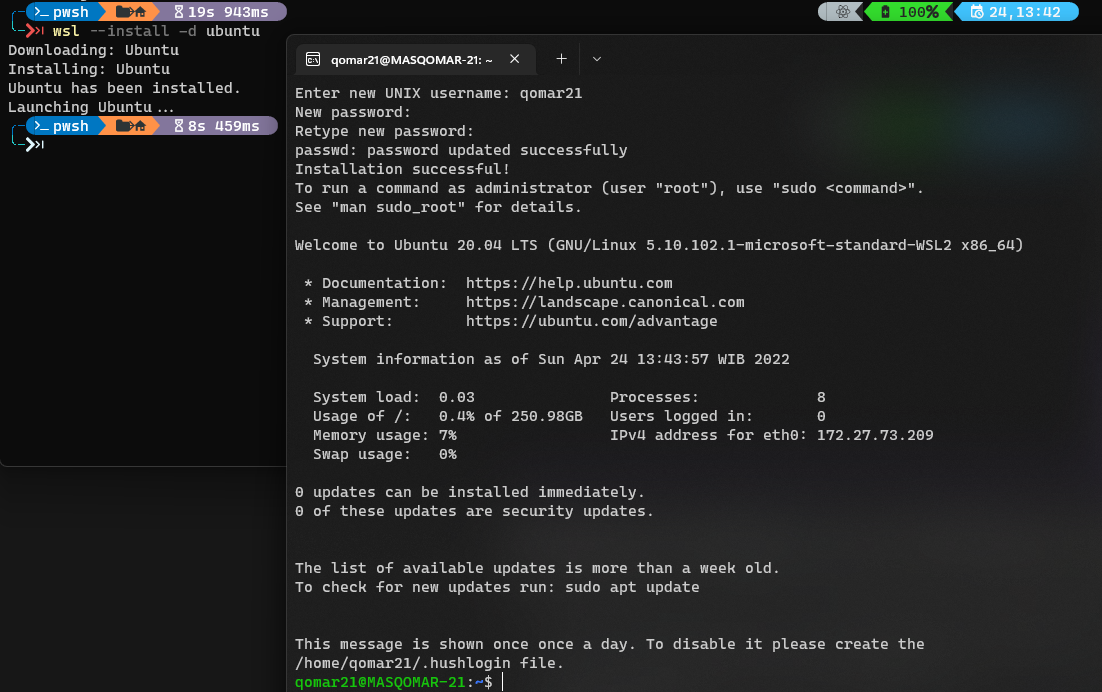
\includegraphics[width=0.7\textwidth]{Figure/asset/install wsl ubuntu.png}
\caption{Install WSL 2 melalui Windows PowerShell}
\end{figure}
selain mengunakan PowerShell, WSL juga dapat diinstall melalui Microsoft Store. dengan cara memasukan kata kunci "wsl" pada lolom Search. kemudian
meilih salah satu disrto yang akan di install, kemudail klik pada "get"
\begin{figure}[h]
\centering
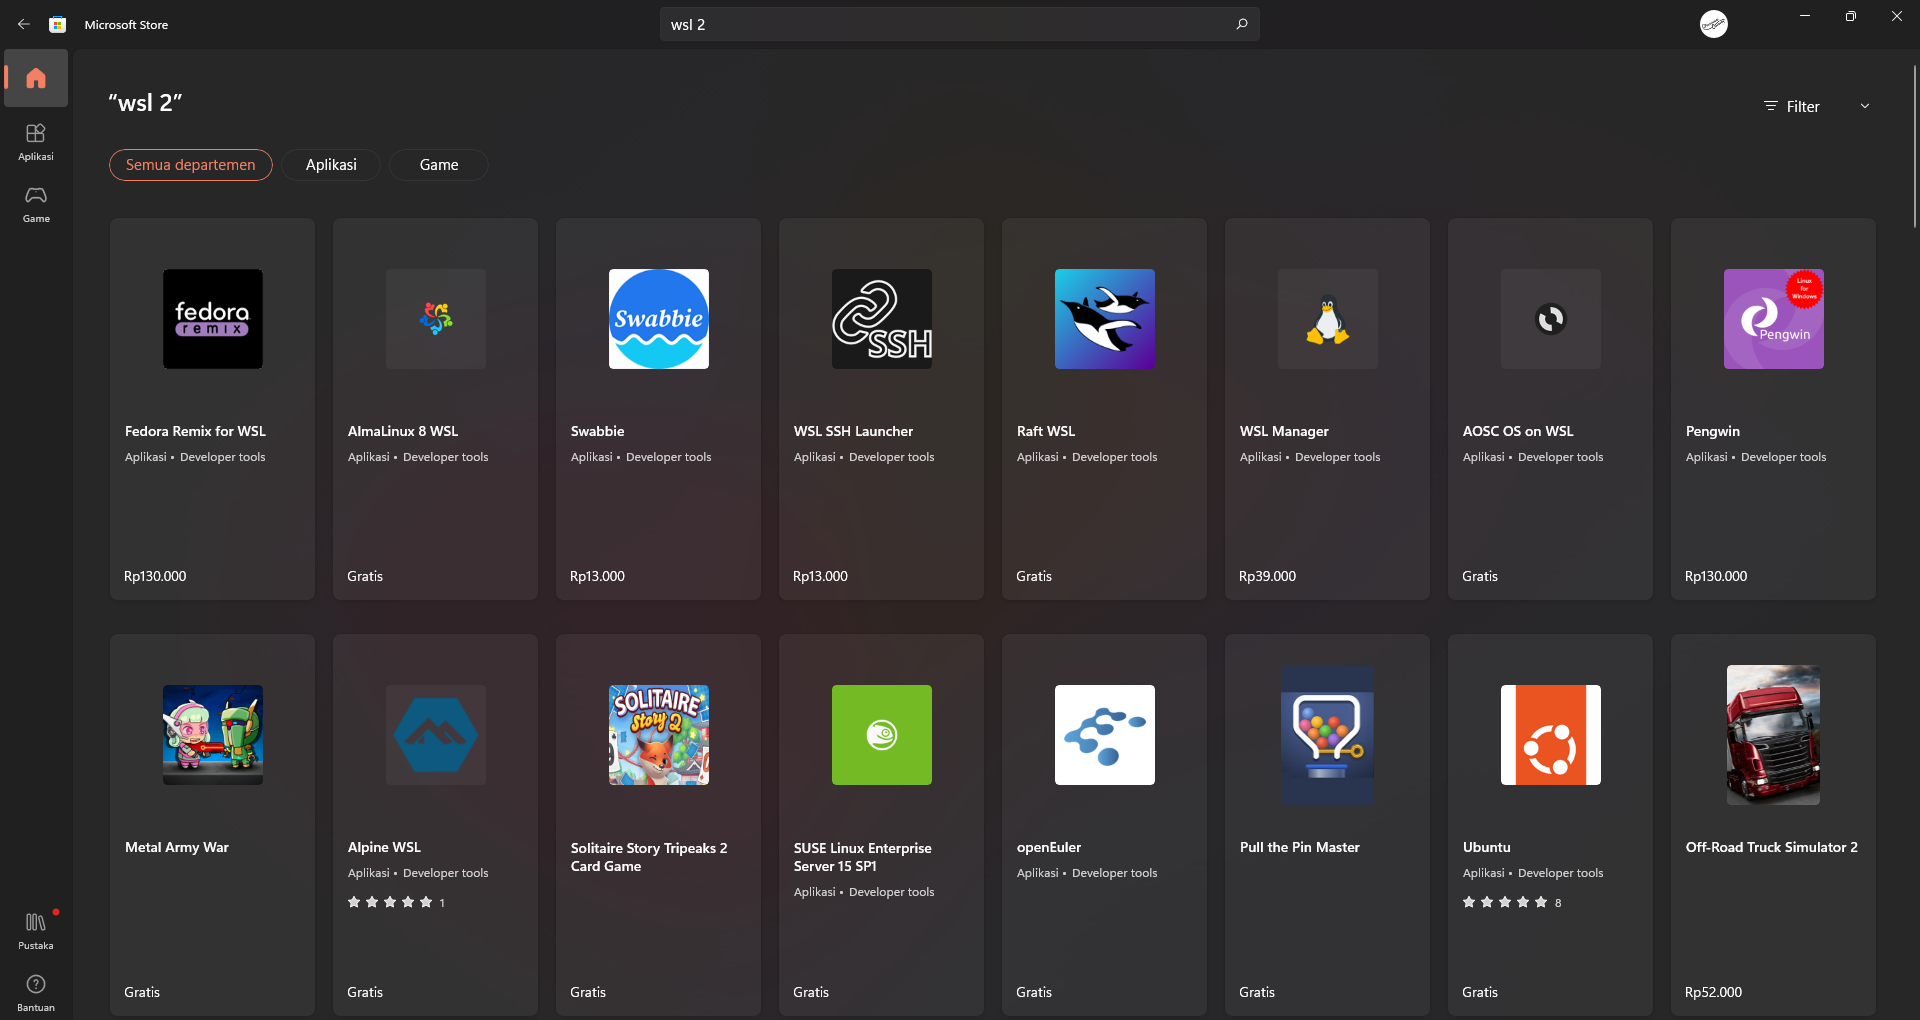
\includegraphics[width=0.7\textwidth]{Figure/asset/wsl from microsoft store.png}
\caption{Install WSL 2 melalui Microsoft Store}
\end{figure}

\subsection{install Docker}
Setelah WSL 2 diinstall, kita bisa menginstall Docker. Dengan cara kita mengunduh file installasi Docker melalui officila website resminya
\href{https://docs.docker.com/desktop/windows/install/}{Docker for Windows}. setelah selesai mengunduh, jalankan file
unduhan yang telah kita unduh tersebut. maka akan muncul Window seperti gambar di bawah ini, kemudain klik "Ok" maka mulai mengunduh
package-package yang diperlukan untuk menginstall Docker.
\begin{figure}[h]
	\centering
	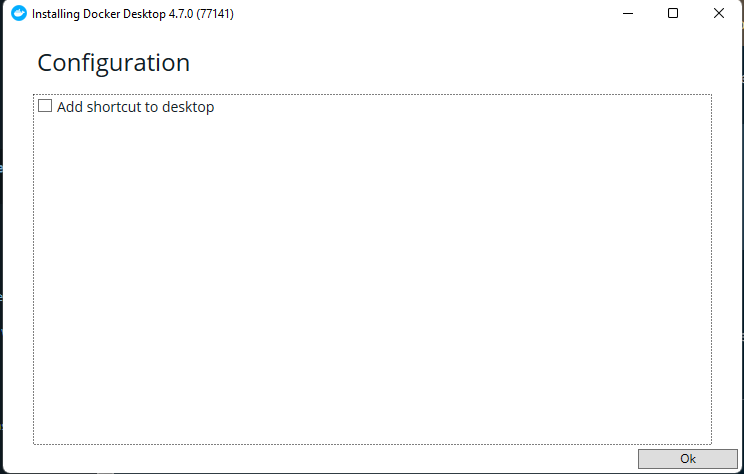
\includegraphics[width=0.7\textwidth]{Figure/asset/1.png}
\end{figure}
\begin{figure}[h]
	\centering
	\begin{subfigure}[b]{0.5\textwidth}
		\centering
		\def\svgwidth{\columnwidth}
		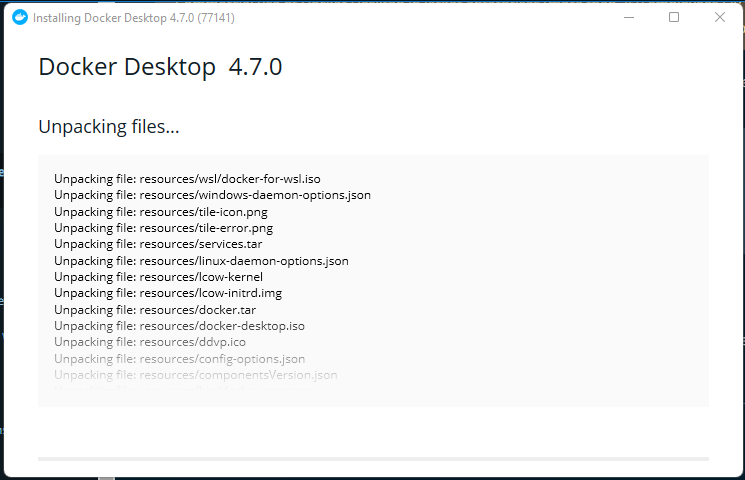
\includegraphics[width=1\textwidth]{Figure/asset/2.png}
	\end{subfigure}
	\begin{subfigure}[b]{0.5\textwidth}
		\centering
		\def\svgwidth{\columnwidth}
		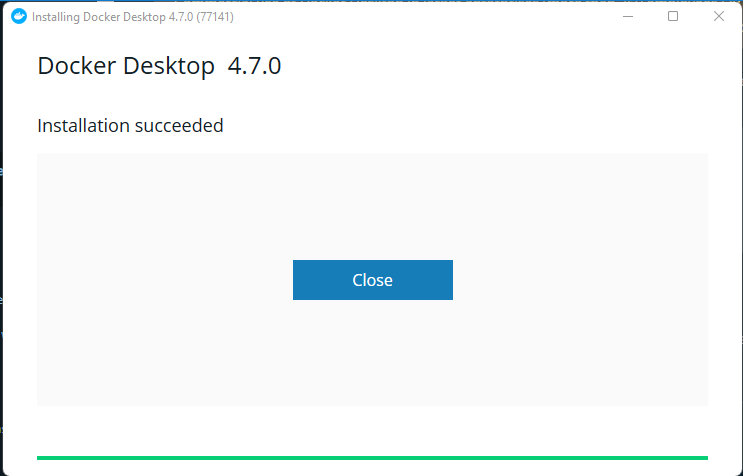
\includegraphics[width=1\textwidth]{Figure/asset/3.png}
	\end{subfigure}
\end{figure}
\newpage
setelah docker terinstall, jalankan Docker tersebut.

\begin{figure}[h]
	\centering
	
\includegraphics[width = 0.5\textwidth]{Figure/asset/4.png}
\end{figure}

kemudian klik "Accept". dan Docker siap di gunakan.

\section{percobaan}

\subsection{Hello-World}
setelah Docker berhasil diInstall, maka kita dapat menjalankan perintah perintah Docker tersebut pada PowerShell atau Command Prompt.
Untuk mengeceknya dapat kita ketikan perintah berikut pada PowerShell
\begin{lstlisting}[language=bash]
	docker run Hello-World
\end{lstlisting}
maka outpunnya akan keluar sebagai berikut
\begin{lstlisting}[language = bash]
	Unabel to find image 'hello-world:latest' locally
	latest: Pulling from library/hello-world
	2db29710123e: Pull complete
	Digest: sha256:10d7d58d5ebd2a652f0d93fdd86da8f265f5318c6a73cc5b6a9798ff6d2b2067
	Status: Downloaded newer image for hello-world:latest

	Hello from Docker!
	This message shows that your installation appears to be working correctly
	....
\end{lstlisting}
\begin{figure}[h]
	\centering
	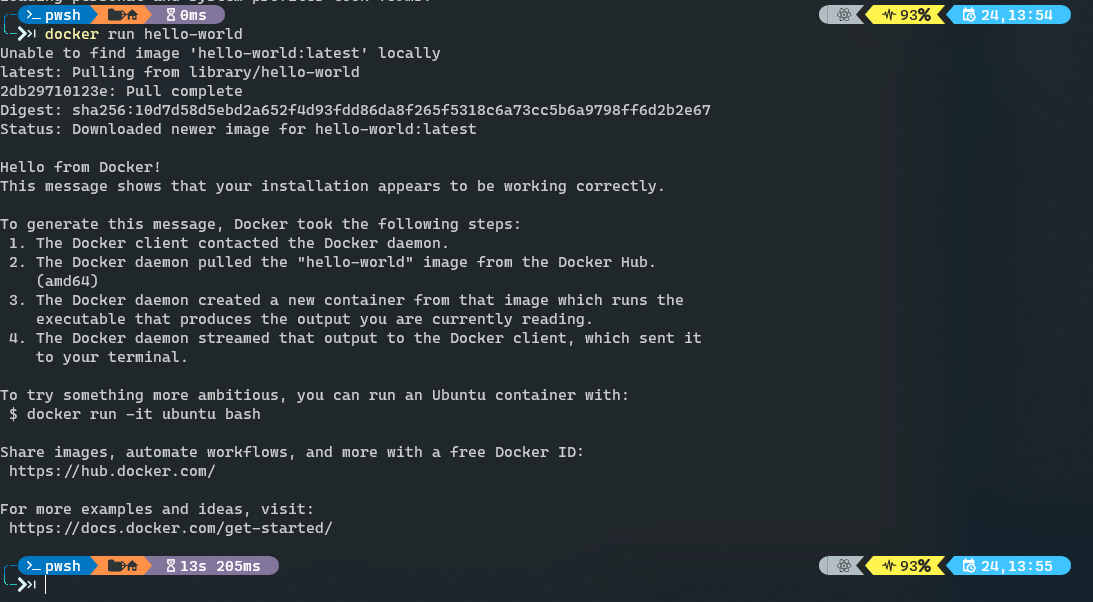
\includegraphics[width = 0.7\textwidth]{Figure/asset/docker_run_helloworld.png}
	\caption{Docker run hello-world}
\end{figure}

\subsection{Alpine linux}
selanjunya kita akan menjalankan image pertama yaitu \textit{alpine linux}.
Untuk menjalankan image tersebut kita perlu mengunduh{pulling} dengan cara mengetikan perintah berikut
\begin{lstlisting}[language = bash]
	Docker Pull Alpine
\end{lstlisting}
\begin{figure}[h]
	\centering
	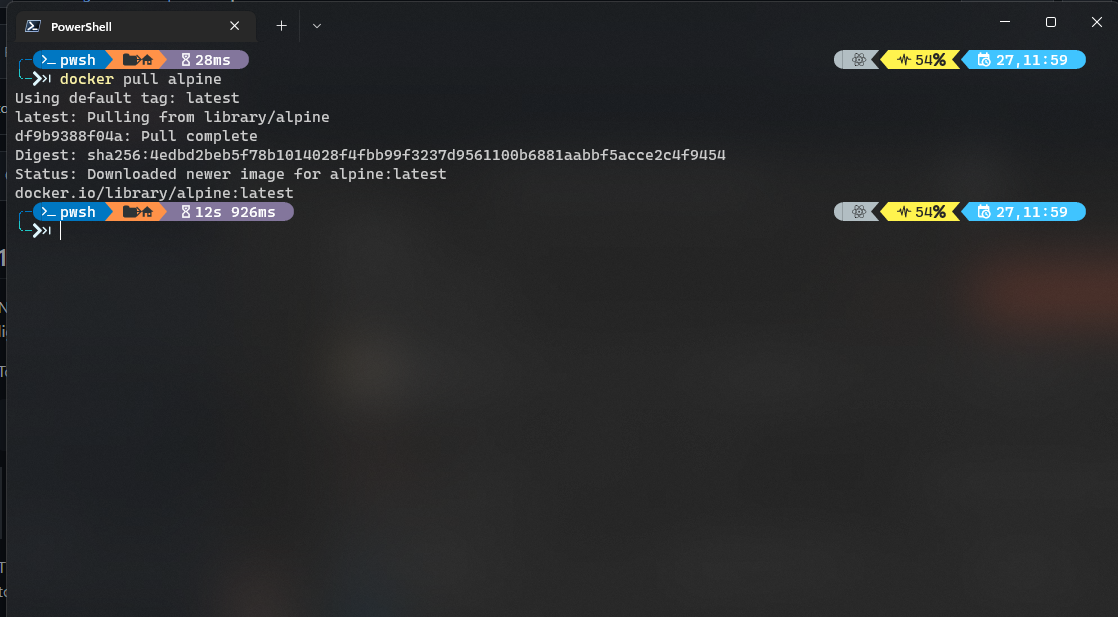
\includegraphics[width = 0.7\textwidth]{Figure/asset/pull_alpine.png}
	\caption{Pulling Alpine Container}
\end{figure}

selanjutnya kita akan mencoba menjalankan salah Container dengan mengetikan perintah berikut
\begin{lstlisting}[language = bash]
	Docker run alpine ls -l
\end{lstlisting}
maka outpunnya sebagi berikut
\begin{figure}[h]
	\centering
	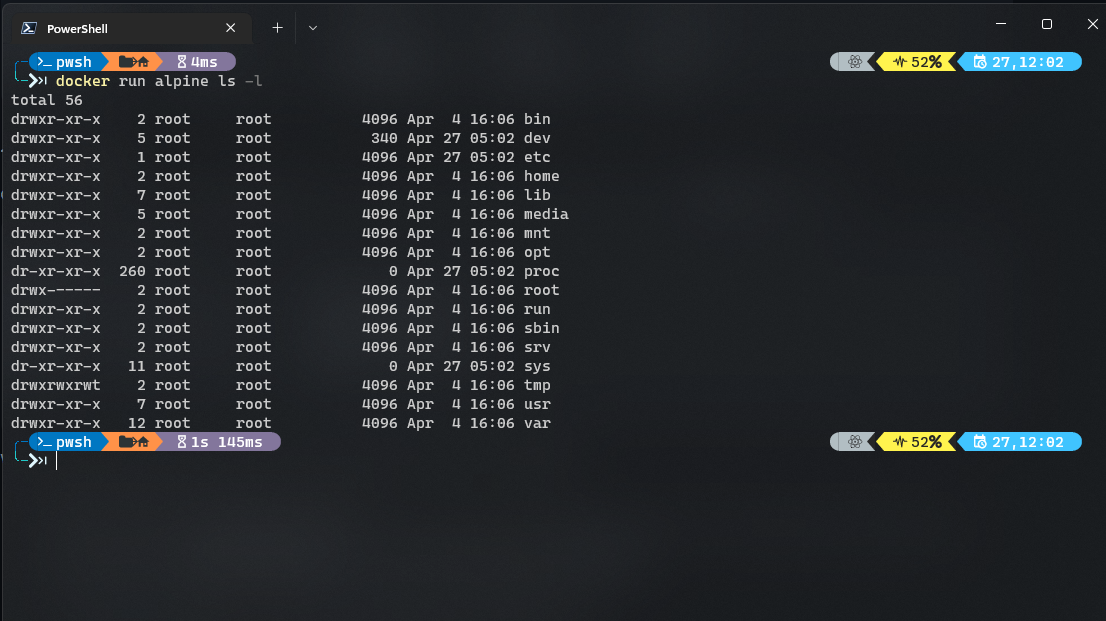
\includegraphics[width = 0.7\textwidth]{Figure/asset/run apline ls -l.png}
	\caption{Docker run alpine ls -l}
\end{figure}

setelah itu kita akan mencoba mengetika "hello from alpine" melalui Container tersebut dengan perintah sebagai berikut
\begin{lstlisting}[language = bash]
	Docker run alpine echo "hello from alpine"
\end{lstlisting} 
maka outpunnya sebagai berikut.
\begin{figure}[h]
	\centering
	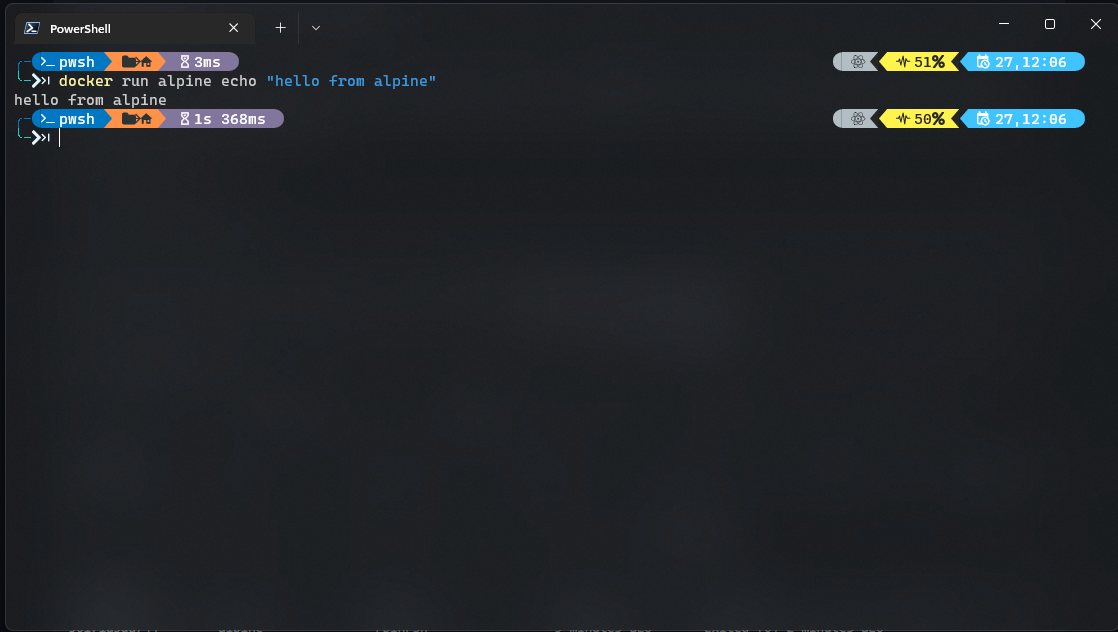
\includegraphics[width = 0.7\textwidth]{Figure/asset/run apline echo.png}
	\caption{Docker run alpine echo}
\end{figure}

\newpage
selanjutnya kita akan mencoba masuk kedalam bash atau Command line dari Container alpine tersebut.
Untuk masuk kedalam kontaner Alpine kita tidak bisa hanya menjalankan Container tersebut dan memberi path untuk bashnya saja.
Tetapi kita juga harus manambah option ketika menjalankan Container tersebut. perintah yang dapat kita gunakan sebagai berikut.
\begin{lstlisting}[language = bash]
	docker run alpine /bin/sh #tidak bisa masuk kedalam bash

	docker run alpine -it /bin/sh 
\end{lstlisting}
seperti tangkap layar berikut.
\begin{figure}[h]
	\centering
	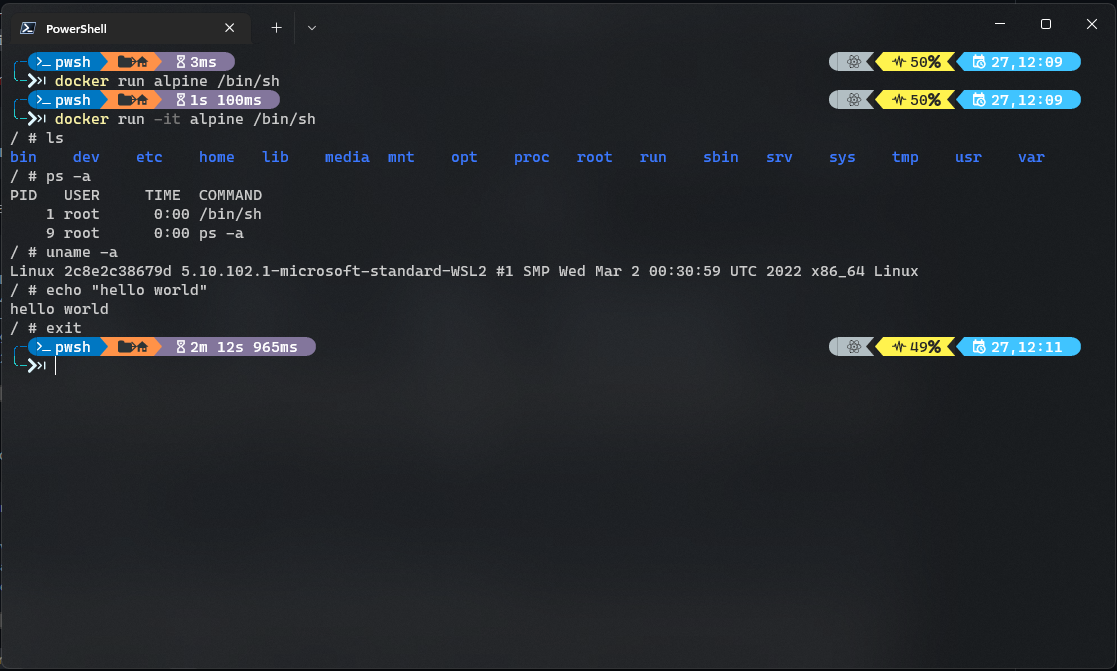
\includegraphics[width = 0.7\textwidth]{Figure/asset/docker_bin_sh.png}
	\caption{masuk bash alpine}
\end{figure}

Option -it berguna untuk masuk dan memberikan perintah pada bash Container tersebut. -i hanya untuk memberikan perintah saja, tetapi tidak akan masuk kedalam bash Container tersebut.
sedangkan -t adalah option untuk masuk kedalam bash Container saja namun tidak dapat memberikan perintah ke dalamnya.\\\\

selanjutnya kita akan mengeceknya Container apa saja yang sudah pernah kita jalankan dengan cara mengetikan perintah berikut.
\begin{lstlisting}[language = bash]
	docker ps -a
\end{lstlisting}
\begin{figure}[h]
	\centering
	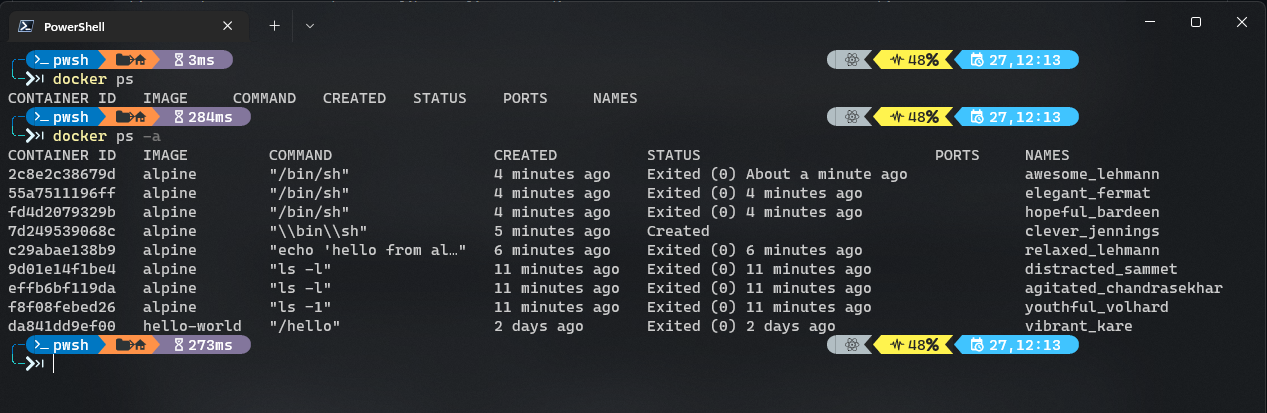
\includegraphics[width = 0.7\textwidth]{Figure/asset/docker ps.png}
	\caption{cek container yang pernah di jalankan}
\end{figure}

selain itu, kita juga dapat mengecek image apa saja ynag pernah kita unduh (pull). dengan mengetikan perintah berikut.
\begin{lstlisting}[language = bash]
	docker images
\end{lstlisting}
\begin{figure}[h]
	\centering
	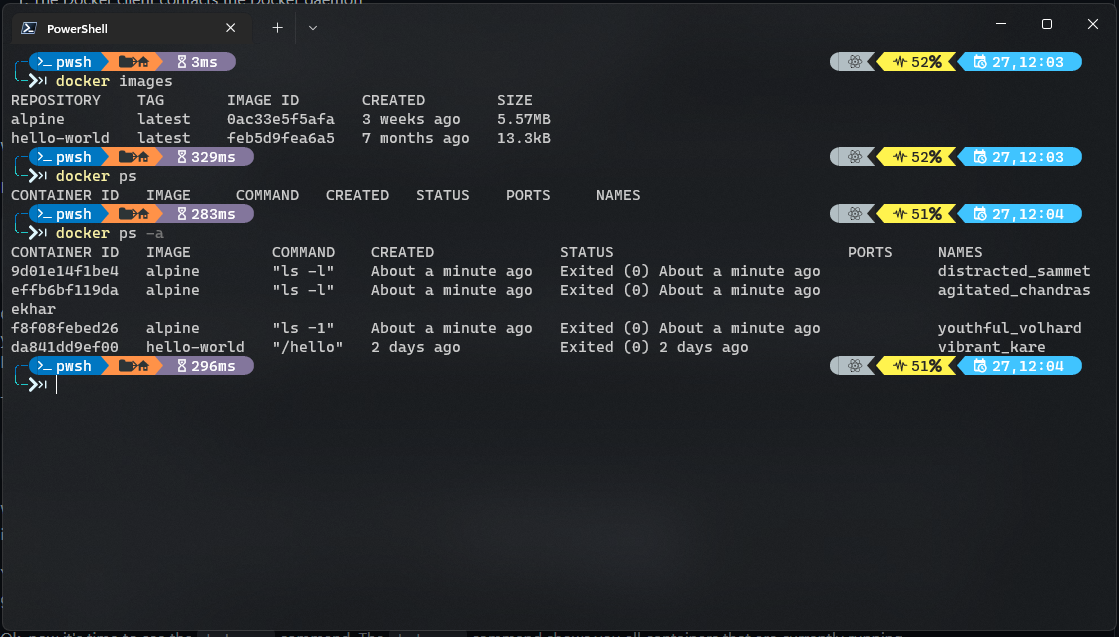
\includegraphics[width = 0.7\textwidth]{Figure/asset/docker_images.png}
	\caption{cek images}
\end{figure}

\section{Jawaban pertanyaan HandsOn}
\subsection*{Apa itu Docker}
Docker merupakan salah satu bentuk virtualisasi yang menungkinkan devloper untuk membuat, 
mengemas, dan menjalankan aplikasi dalam sebuah Container. Docker sebenarnya mirip dengan 
Vitrual Mecine (VM), karena kedaunya sama sama memerlukan \textit{resouce isolation} yang artinya
sama sama mengisolasi sumber daya untuk dapat di jalankan. namun, Docker dan VM memeiliki
perbedaan yang moncolok, yaitu pada resouce yang di perlukan. sebagai ilustrasi, pada saat 
menjalankan sebuah aplikasi dengan menggunakan Virtual Mecine, maka kita perlu menyiapkan 
sistem opreasi yang lengkap yang mana akan membutukan resoure yang cukup besar. berbeda dengan
menggunakan Docker, kita tidak perlu menyiapkan seluruh sistem operasi yang lengkap, kita hanya
perlu menyiapkan hal hal yang kita perlukan dalam aplikasi tersebut, sehingga resouce yang kita 
perlukan juga akan lebih sedikit. Hal ini dapat terjadi karena Docker memanfaatkan Kernel Linux
pada level Host OS untuk di gunakan secara bersama-sama (Shere) oleh container.


\subsection*{apa fungsi perintah "docker run"}

\subsection*{Apa itu Conatainer}

\subsection*{apa fungsi perintah "docker run -it"}

\subsection*{Apa itu images}

\subsection*{Apa itu deamon}













\end{document}